\section{Homework 3}

\subsection{Graphical Density}
(a) We have
\[
2\cdot1\cdot A + 1\cdot1\cdot (2A) + 2\cdot1\cdot A = 1,
\]
so $A = \frac{1}{6}$. Below we sketch the p.d.f.'s for $f_X$, $f_Y$, and $f_{X|X+Y\leq3}$, respecitvely:

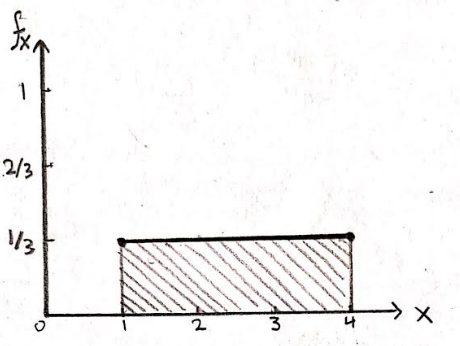
\includegraphics[scale=0.3]{f_X}
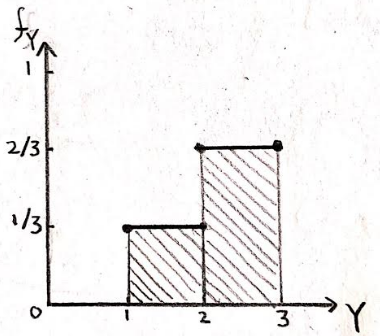
\includegraphics[scale=0.3]{f_Y}
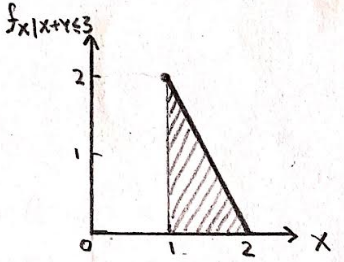
\includegraphics[scale=0.4]{f_conditional}

(b) For $\E[X|Y = y]$, we have symmetry on both $[1, 2]$ and $[2, 3]$ around $X = 2.5$. Thus $\E[X|Y = y] = 2.5$ for $1 \leq y \leq 3$.

On the other hand, for $\E[Y|X = x]$ is less symmetric, and we have the piecewise function:
\[
\E[Y|X = x] = 
\begin{cases}
    2 &\f{if } 1 \leq x \leq 2 \\
    2.5 &\f{if } 2 < x \leq 3 \\
    2 &\f{if } 3 < x \leq 4.
\end{cases}
\]

(c) From the previous part, we have $\E[X] = 5/2$, and $\E[Y] = (1/3)(2 + 5/2 + 2) = 13/6$. Now, we just need to find
\begin{align*}
    \E[XY] &= \int_1^3\int_1^2 \frac{xy}{6} dxdy + \int_2^3\int_2^3 \frac{xy}{3}dxdy + \int_1^3\int_3^4 \frac{xy}{6}dxdy \\
    &= 1 + \frac{25}{12} + \frac{7}{3} \\
    &= \frac{65}{12}.
\end{align*}
Thus we have that
\begin{align*}
\f{Cov}(X, Y) &= \E[XY] - \E[X]\E[Y] \\
&= \frac{65}{12} - \left(\frac{5}{2}\right)\left(\frac{13}{6}\right) \\
&= 0.
\end{align*}

\subsection{Conditional Distribution of a Poisson Random Variable with Exponentially Distributed Parameter}

(a) Integrating by parts, we get a recurrence relation, which we can exploit to get
\begin{align*}
    \E[\lambda^k] &= \int_0^\infty x^k f_\lambda(x) dx \\
    &= \int_0^\infty x^k\theta e^{-\theta x} dx \\
    &= \left.\left(-x^k e^{-\theta x}\right)\right|_{0 \f{ to } \infty} + \int_0^\infty kx^{k-1}e^{-\theta x} dx \\
    &= k\int_0^\infty x^{k-1}e^{-\theta x} dx \\
    &\quad\vdots \\
    &= \frac{k!}{\theta^{k-1}}\int_0^\infty e^{-\theta x} dx \\
    &= \frac{k!}{\theta^{k-1}}\left.\left(\frac{e^{-\theta x}}{-\theta}\right)\right|_{0 \f{ to } \infty} \\
    &= \frac{k!}{\theta^k},
\end{align*}
which is what we wanted.

(b) Using a similar approach to the previous part, we get an integral by parts and a recurrence relation which we exploit to get
\begin{align*}
    \P[X = k] &= \int_0^\infty e^{-x}\frac{x^k}{k!}f_\lambda(x) dx \\
    &= \frac{\theta}{k!}\int_0^\infty e^{-(\theta + 1)x}x^k dx \\
    &= \frac{\theta}{k!}\left(\left.\frac{-x^k e^{-(\theta + 1)x}}{\theta + 1}\right|_{o \f{ to } \infty} + \frac{k}{\theta + 1}\int_0^\infty x^{k-1}e^{-(\theta + 1)x} dx \right) \\
    &= \frac{\theta}{k!}\left(\frac{k}{\theta + 1}\int_0^\infty x^{k-1}e^{-(\theta + 1)x} dx \right) \\
    &\quad\vdots \\
    &= \frac{\theta}{k!}\left(\frac{k!}{(\theta + 1)^{k+1}}\right) \\
    &= \left(\frac{1}{\theta + 1}\right)^k\left(\frac{\theta}{\theta + 1}\right).
\end{align*}
Thus, $X$ is geometric (albeit shifted left by 1, i.e. with support $\N \cup \{0\}$) with parameter $p = \frac{\theta}{\theta + 1}$.

(c) Using Bayes' Rule and our result from the previous parts, we obtain:
\begin{align*}
    f_{\lambda|X}(\mu | X = k) &= \frac{f_\lambda(\mu) \cdot \P[X = k | \lambda = \mu]}{\P[X = k]} \\
    &= \frac{\left(\theta e^{-\theta\mu}\right)\left(e^{-\mu}\frac{\mu^k}{k!}\right)}{\left(\frac{1}{\theta + 1}\right)^k\left(\frac{\theta}{\theta + 1}\right)} \\
    &= \frac{e^{-(\theta + 1)\mu}\mu^k}{k!(\theta + 1)^{k+1}}.
\end{align*}

\subsection{Gaussian Densities}
(a) Let $Z = X_1 + X_2$. Then we have the convolution:
\begin{align*}
    f_Z(z) &= \int_{-\infty}^\infty f_{X_1}(t)f_{X_2}(z - t) dt \\
        &= \int_{-\infty}^\infty \frac{1}{\sigma_1\sigma_2 2\pi} e^{-\left(\frac{t^2}{2\sigma_1^2} + \frac{(z - t)^2}{2\sigma_2^2}\right)} dt \\
        &= \int_{-\infty}^\infty \frac{1}{\sqrt{2\pi}\sqrt{\sigma_1^2 + \sigma_2^2}} \cdot \frac{1}{\sqrt{2\pi}\frac{\sigma_1\sigma_2}{\sqrt{\sigma_1^2 + \sigma_2^2}}} e^{-\left(\frac{\sigma_2^2t^2 + \sigma_1^2t^2 - 2zt\sigma_1^2 + z^2\sigma_1^2}{2\sigma_1^2\sigma_2^2}\right)} dt \\
        &= \frac{1}{\sqrt{2\pi}\sqrt{\sigma_1^2 + \sigma_2^2}} \int_{-\infty}^\infty \frac{1}{\sqrt{2\pi}\frac{\sigma_1\sigma_2}{\sqrt{\sigma_1^2 + \sigma_2^2}}} e^{-\left(\frac{(\sigma_1^2 + \sigma_2^2)\left(t - \frac{\sigma_1^2z}{\sigma_1^2 + \sigma_2^2}\right)^2 - \frac{\sigma_1^4z^2}{\sigma_1^2 + \sigma_2^2} + z^2\sigma_1^2}{2\sigma_1^2\sigma_2^2}\right)} dt \\
        &= \frac{1}{\sqrt{2\pi}\sqrt{\sigma_1^2 + \sigma_2^2}} e^{-\frac{z^2}{2(\sigma_1^2 + \sigma_2^2)}}\int_{-\infty}^\infty \frac{1}{\sqrt{2\pi}\frac{\sigma_1\sigma_2}{\sqrt{\sigma_1^2 + \sigma_2^2}}} e^{-\frac{t^2}{2\left(\frac{\sigma_1\sigma_2}{\sqrt{\sigma_1^2 + \sigma_2^2}}\right)^2}} dt \\
        &= \frac{1}{\sqrt{2\pi}\sqrt{\sigma_1^2 + \sigma_2^2}} e^{-\frac{z^2}{2(\sigma_1^2 + \sigma_2^2)}}.
\end{align*}
Notice the expression in the integral is just integrating the pdf of a gaussian random variable, so it evaluates to 1, giving us the pdf of $Z = X_1 + X_2$, which is just that of $\mathcal{N}(0, \sigma_1^2 + \sigma_2^2)$.

(b) First, notice that if we add together two gaussian rv's with nonzero mean, the mean pops out as a scalar translation of the combined random variable. In particular, if we have $X_1 \sim \mathcal{N}(\mu_1, \sigma_1^2)$ and $X_2 \sim \mathcal{N}(\mu_2, \sigma_2^2)$, then $X_1 = Y_1 + \mu_1$ and $X_2 = Y_2 + \mu_2$, where $Y_i \sim \mathcal{N}(0, \sigma_i^2)$. It follows then that $X_1 + X_2 = Y_1 + Y_2 + (\mu_1 + \mu_2)$. Then any linear combination of i.i.d. gaussian random variables $\mathcal{N}(\mu, \sigma^2)$ will come out to be
\[
    \sum_{i = 1}^n c_iX_i = \sum_{i = 1}^n Y_i + \sum_{i = 1}^n c_i\mu,
\]
where $Y_i \sim \mathcal{N}(0, c_i^2\sigma^2)$. By our result from part (a), we get then a gaussian random variable
\[
    Z \sim \mathcal{N}(\sum_{i = 1}^n c_i\mu, \sum_{i = 1}^n c_i^2\sigma^2).
\]
Thus any linear combination of finitely many i.i.d. gaussian random variables is also gaussian.

(c) First, note that if $n$ is odd, we have the integral
\[
    \int_{-\infty}^\infty x^n \frac{1}{\sqrt{2\pi}\sigma}e^{-\frac{x^2}{2\sigma^2}} dx,
\]
which evaluates to 0 since we have an odd function over the real line.

So suppose $n$ is even. Then we integrate by parts to get
\begin{align*}
    \E[X^n] &= \int_{-\infty}^\infty x^n \frac{1}{\sqrt{2\pi}\sigma}e^{-\frac{x^2}{2\sigma^2}} dx \\
        &= \frac{1}{\sqrt{2\pi}\sigma} \int_{-\infty}^\infty x^{n - 1} xe^{-\frac{x^2}{2\sigma^2}} dx \\
        &= \frac{1}{\sqrt{2\pi}\sigma} \left(\left.-\sigma^2x^{n - 1}e^{-\frac{x^2}{2\sigma^2}}\right|_{-\infty \f{ to } \infty} - \int_{-\infty}^\infty -\sigma^2(n - 1)x^{n - 2}e^{-\frac{x^2}{2\sigma^2}} dx\right) \\
        &= \frac{1}{\sqrt{2\pi}\sigma}\int_{-\infty}^\infty \sigma^2(n - 1)x^{n - 2}e^{-\frac{x^2}{2\sigma^2}} dx \\
        &= \frac{\sigma^2(n - 1)}{\sqrt{2\pi}\sigma}\int_{-\infty}^\infty x^{n - 2}e^{-\frac{x^2}{2\sigma^2}} dx \\
        &\quad\vdots \\
        &= \frac{\sigma^n n!}{\sqrt{2\pi}\sigma 2^{n/2}(n/2)!} \int_{-\infty}^\infty e^{-\frac{x^2}{2\sigma^2}} dx \\
        &= \frac{\sigma^n n!}{2^{n/2}(n/2)!}
\end{align*}

(d) First, we find the means:
\begin{align*}
    \E[Z] &= 0 \\
    \E[I\{Z > c\}] &= \int_c^\infty \phi(x)dx \\
        &= 1 - \Phi(c),
\end{align*}
which gives us the mean vector $(0, 1 - \Phi(c))$. Now, we compute the covariances:
\begin{align*}
    \f{Cov}(Z, Z) &= \f{Var}(Z) = 1 \\
    \f{Cov}(I, I) &= \E[I^2] - \E[I]^2 \\
        &= (1 - \Phi(c)) - (1 - \Phi(c))^2 \\
        &= \Phi(c) - \Phi(c)^2 \\
    \f{Cov}(Z, I) &= \f{Cov}(I, Z) \\
        &= \E[ZI] - \E[Z]\E[I] \\
        &= \int_c^\infty x\phi(x) dx \\
        &= \int_c^\infty \frac{x}{\sqrt{2\pi}}e^{-\frac{x^2}{2}} dx \\
        &= \frac{1}{\sqrt{2\pi}}(-e^{-\frac{x^2}{2}})\mid_{c \f{ to } \infty} \\
        &= \frac{e^{-\frac{c^2}{2}}}{\sqrt{2\pi}}.
\end{align*}
Putting these together, we get the covariance matrix:
\[
\left[\begin{tabular}{cc}
    1 & $\frac{e^{-\frac{c^2}{2}}}{\sqrt{2\pi}}$ \\
    $\frac{e^{-\frac{c^2}{2}}}{\sqrt{2\pi}}$ & $\Phi(c) - \Phi(c)^2$
\end{tabular}\right]
\]

\subsection{Joint Density for Exponential Distribution}
(a) We get the double integral and evaluate:
\begin{align*}
    \P[X < Y] &= \int_0^\infty \int_x^\infty f_X(x)f_Y(y) dydx \\
        &= \lambda\mu\int_0^\infty \int_x^\infty e^{-\lambda x}e^{-\mu y}dydx \\
        &= \lambda\mu\int_0^\infty\frac{e^{-(\lambda + \mu)x}}{\mu} dx \\
        &= \frac{\lambda}{\lambda + \mu}.
\end{align*}

(b) First, we find $\P[X_j > t]$ given $t > 0$. This is
\[
\P[X_j > t] = \int_t^\infty\lambda_je^{-\lambda_jx}dx = e^{-\lambda_jt}.
\]
Now, since the $X_k$'s are independent, we have
\begin{align*}
    \P[X_i = \min_{1 \leq k \leq n}X_k] &= \int_0^\infty f_{X_i}(t)\prod_{j \neq i}\P[X_j > t]dt \\
    &= \int_0^\infty \lambda_i\prod_k e^{-\lambda_k t} dt \\
    &= \left.\left(\frac{\lambda_i e^{-(\sum \lambda_k)t}}{-\sum \lambda_k}
\right)\right|_{0 \f{ to } \infty} \\
    &= \frac{\lambda_i}{\sum_{k = 1}^n \lambda_k},
\end{align*}
which is what we wanted.

\subsection{Matrix Sketching}
(a) First, we compute the mean matrix. Note that since the $S_{ij}$'s are independent and standard normal random variables, the value of $\E[S_{i_1j_1}S_{i_2j_2}] = \E[S_{i_1j_1}]\E[S_{i_2j_2}] = \mu_1\mu_2$ is just 0. Then the only elements of $S^TS$ that are nonzero are the ones along the diagonal. In particular, the $k$th element along the diagonal will be
\begin{align*}
    \frac{1}{d}\left(\E\left[\sum_{i = 1}^dS_{ik}\right]\right) &= \E[S_1k^2] \\
    &= 1,
\end{align*}
by plugging in 2 to our $n$th moment formula for $\E[X^n]$ from problem 3(c). Thus the mean matrix is simply $I_n$, the $n \times n$ identity matrix.

Now, we compute the variance matrix. First, for any two independent random variables $X$ and $Y$, the variance of their product will be
\begin{align*}
    \f{Var}(XY) &= \E[X^2Y^2] - \E[XY]^2 \\
    &= \E[X^2]\E[Y^2] - \E[X]^2\E[Y]^2 \\
    &= \f{Var}(X)\f{Var}(Y) + \f{Var}(X)\E[Y]^2 + \f{Var}(Y)\E[X]^2.
\end{align*}
So, when we compute the value of non diagonal elements, we get
\begin{align*}
    \f{Var}\left(\frac{1}{d}\sum_{i = 1}^d S_{ij}S_{ik}\right) &= \frac{1}{d}\f{Var}(S_{1j}S_{1k}) \\
    &= \frac{1}{d}(1 \cdot 1 + 1 \cdot 0 + 1 \cdot 0) \\
    &= 1/d.
\end{align*}
Now, we consider elements along the diagonal. Using independence, we get
\begin{align*}
    \f{Var}\left(\frac{1}{d}\sum_{i = 1}^d S_{ij}S_{ij}\right) &= \frac{1}{d}\f{Var}(S_{1j}^2) \\
    &= (\frac{1}{d}(\E[S_{1j}^4] - \E[S_{1j}^2]^2) \\
    &= \frac{1}{d}(3 - 1) \\
    &= 2/d,
\end{align*}
where the last line was obtained using our formula for $\E[X^n]$ from problem 3(c). Thus our variance matrix is an $n \times n$ matrix with $(2/d)$'s along the diagonal and $(1/d)$'s everywhere else.

(b) First, we find the mean matrix. For non-diagonal elements, we have
\begin{align*}
    \E\left[\sum_{i = 1}^d S_{ij}S_{ik}\right] &= \sum_{i = 1}^d\E[S_{ij}S_{ik}] \\
    &= 0,
\end{align*}
by symmetry of positives and negatives. Now, for diagonal elements, we have
\begin{align*}
    \E\left[\sum_{i = 1}^d S_{ij}S_{ij}\right] &= \sum_{i = 1}^d\E[S_{ij}^2] \\
    &= d\left(\frac{1}{2d}(1)^2 + \frac{1}{2d}(-1)^2\right) \\
    &= 1.
\end{align*}
Thus our mean matrix is just $I_n$, the $n \times n$ identity matrix.

Now, we compute the variance matrix. For non-diagonal elements, $\E[X]$ is just 0 from above, so we only need to find $\E[X^2]$, or the expected value of the square of the dot product. There is a $1/d$ chance that the $\pm 1$ of each vector aligns (otherwise the dot product would just be 0), and since we are squaring the parity is irrelevant. Therefore $\E[X^2] = 1/d$, which is our non-diagonal variance. For elements along the diagonal, notice that the dot product will always evaluate to 1, and so the variance there is 0. Thus, our variance matrix is an $n \times n$ matrix with 0's along the diagonal and $1/d$ everywhere else.



\subsection{Records}
(a) Since $X_1$ and $X_2$ are i.i.d., we note that by symmetry,
\begin{align*}
\P[X_1 > X_2] + \P[X_2 > X_1] &= 1 \\
\P[X_2 > X_1] &= 1/2,
\end{align*}
so $X_2$ is a record-to-date with probability 1/2.

(b) Since the probability that any two $X_i$'s coincide is zero (by the nature of continuous probability), we can treat the event that $X_n$ is a record-to-date as the event where $X_n = \max_{1 \leq i \leq n}X_i$. By symmetry, we get that this probability is simply $1/n$.

(c) We split the expectation into indicator random variables $I_k$ each denoting whether or not the $k$th trial was a record-to-date. Thus by linearity, we have
\[
\E[X] = \E\left[\sum_{k = 1}^n I_k\right] = \sum_{k = 1}^n\E[I_k] = \sum_{k = 1}^n \frac{1}{k} \approx \ln n,
\]
which, as we take the limit $n \to \infty$, goes to $\infty$.